\chapter{Linear Models and Estimation by Least Squares}
\section{Introduction} We are going to do best-fit lines in 2 separate ways.

\nl Consider some sample (data) $S = \{(x_i,\, y_i)\}$. In the background, there can be an underlying joint PDF $f(x,y)$
\begin{center}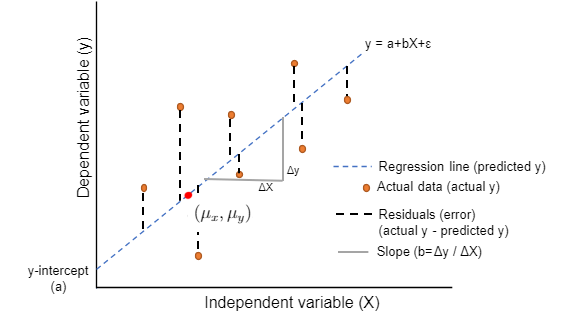
\includegraphics[width=4in]{ch11_regression.png}\end{center}
\section{Linear Statistical Models}

\noindent Assumptions
\begin{enumerate}[label=\textcircled{\raisebox{-1pt}{\arabic*}}]
    \item $Y$ is dependent upon $X$. (i.e. not an independent random variable.)
    \item In general, $y = mx + b$, the general relationship between $X$ and $Y$.
\end{enumerate} 

\newpage
\section{The Method of Least Squares}
\nl\textbf{A.) The probabalistic construction:}

\nl Given all possible lines $y=mx+b$ that \textit{could} describe the data, the \say{most likely} one will be a line that intersects the point $(\mu_x, \mu_y)$.

\nl That is $y - \mu_y = m(x-\mu_x)$. Because we are interpreting $y$ and a function of $x$, the \say{best line} should be one that minimizes the vertical distance (error (residuals)) in the $y$-direction.

\nl For a point $(x_k,\, y_k)$ in $S$, the vertical distaince is 
$$\text{dist} = \abs{y_k - \big(m(x_k - \mu_x) + \mu_y \big)}.$$
Minimizing absolute values is a pain, but calculus I suggests we square this,
$$\operatorname{dist}^2 = \Big((y_k-\mu_y) - m(x_k-\mu_x)\Big)^2.$$
As $x,y$ are distributed via some PDF, the best way to compute our minimization problem is to minimize expectation with respect to slope $m$:
$$K(m) := \E{\operatorname{dist}^2(m)} = \underbrace{\E{\Big((y_k-\mu_y) - m(x_k-\mu_x)\Big)^2}}_{\setRed **}.$$
\setRed ** \setBlack The $m$ that minimizes is called the solution to our \underline{least-squares problem}.
\begin{align*}
    K(m) &= \E{(y_k-\mu_y)^2  -2m(x_k-\mu_x)(y_k - \mu_y) + m^2(x_k-\mu_x)^2 }\\
    &= \E{(y_k-\mu_y)^2} -2m \E{(x_k-\mu_x)(y_k - \mu_y) } + m^2\E{(x_k-\mu_x)^2}\\
    &= S^2_y - 2m \Cov(X,Y) + m^2S^2_x
\end{align*}
Minimizing (with respect to $m$) $\dfrac{\partial}{\partial m}$,
$$K'(m) = -2 \Cov(X,Y) - 2mS^2_x.$$
With $K'(m) = 0$ then $m = \dfrac{\Cov(X,Y)}{S^2_x}$. 

\nl Note that by the second derivitive test, $K''(m) = 2S_x^2 > 0$. In AP Stats (MTH 111), the slope is moved to a \say{prettier} form:

\begin{align*}
    m &= \frac{\Cov(X,Y)}{S_x^2} \\
    &= \frac{\Cov(X,Y)}{S_x S_y} \cdot \frac{S_y}{S_x}\\
    &= \rho \cdot \frac{S_y}{S_x} \hspace{1in} \rho := \frac{\Cov(X,Y)}{S_xS_y}
\end{align*}

\nl \bu{FACT \#1}: The sign of the slope depends entirely upon $\rho$, where the sign is dependent upon $\Cov(X,Y)$

\nnl \bu{FACT \#2}: $-1 \leq \rho \leq 1$.

\nl (For my MTH 325 class, we proved this fact in full generality).

\nnl \bu{FACT \#3}: The closer $\abs{\rho}$ is to 1, the better the line $\widehat{y} = mx+b$ \say{fits} the data.
\begin{center}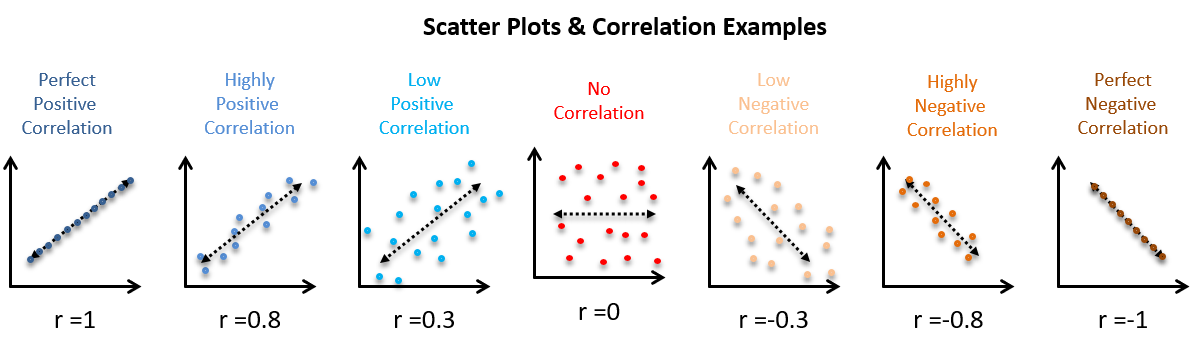
\includegraphics[width=6in]{ch11_scatter.png}\end{center}

\nl The AP Stats definition fo the best fit line is $\widehat{y} = \widehat{b}_0 + \widehat{b}_1x$ where $\widehat{b}_1 = \rho \dfrac{S_y}{S_x}$ and $\widehat{b}_0 = \bar{y} - \widehat{b}_1 \bar{x}$.

\nnl\textbf{B.) The linear algebra construction:}

\nl We still have $S = \{(x_k,\, y_k)\}$. We want $y = mx+b$. Using $S$ always yields an overdetermined (i.e. inconsistent) system
\begin{align*}
    y_1 &= mx_1 + b\\
    y_2 &= mx_2 + b\\
    & \;\;\vdots\\
    y_n &= mx_n + b.
\end{align*}
This is $n$ equations with 2 variables, but we can rewrite as vector equations. $$\vec{y} = m\vec{x} + b \vec{1} \quad \text{where } \vec{y} = \thru{y}, \vec{x} = \thru{x}, \text{ and } \vec{1} = \underbrace{(1,1,\dots,1)}_{n \text{ components}}.$$

\nl Trying to write $\vec{y}$ as a linear combination of $\vec{x}$ and $\vec{1}$. Consider the plane $P = \operatorname{span}\{\vec{x},\vec{1}\}$. Inconsistent implies that $\vec{y} \not \in P$.

\nl But the vector in $P$ that is closest to $\vec{y}$ is $\operatorname{proj}_P\vec{y}$. (Closest under Euclidean distance), recall $\inner{u,v} = u \cdot v$ in $\R^n$.
$$\operatorname{dist}^2 = \sum (y_i - v_i)^2, \quad \vec{v} \in P = \underbrace{\vec{y} \cdot \vec{v} = \inner{y,v}}_{\substack{\text{\say{least squares}}}}$$
\begin{center}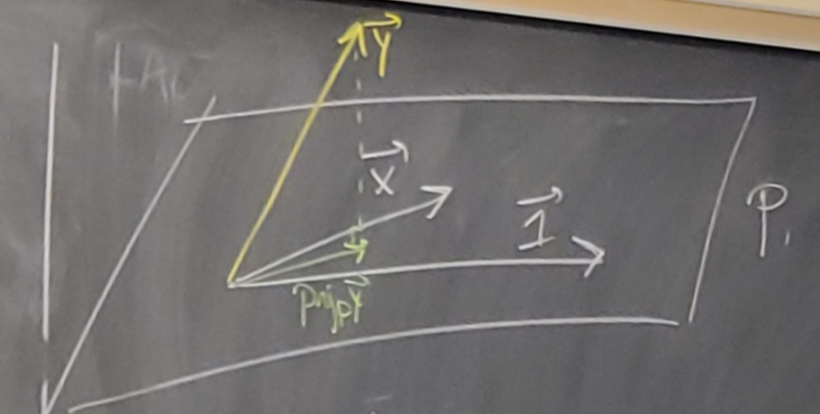
\includegraphics[width=4in]{ch11_proj.png}\end{center}

\noindent Easiest way to project onto $P$ is to have an orthogonal basis for $P$. We need an orthogonal basis for $P$: 
\begin{center}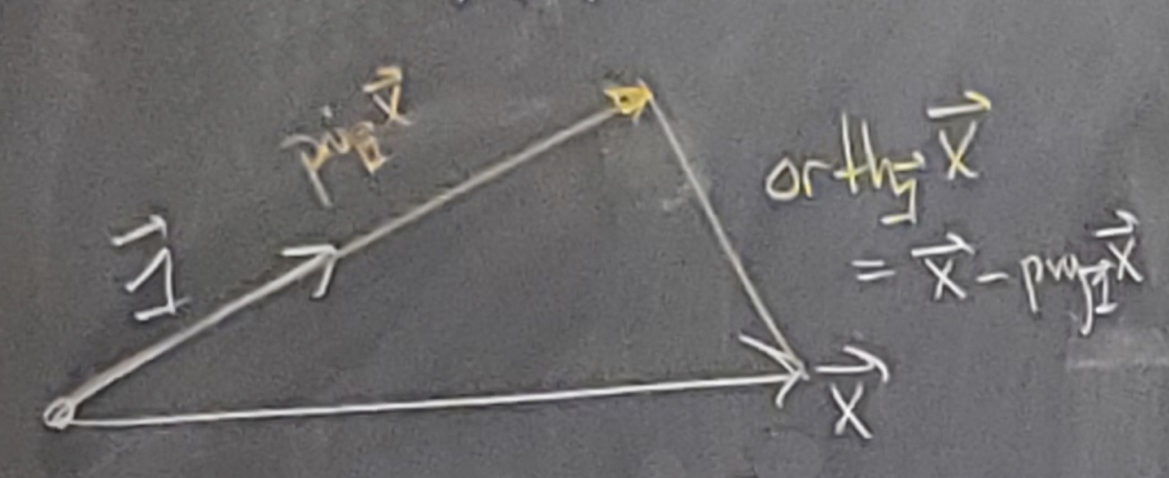
\includegraphics[width=4in]{ch11_basis.png}\end{center}

\nl $P = \operatorname{span}\left\{1, \, \operatorname{orth}_{1}x \right\} = \operatorname{span}\left\{1,\, v\right\}$ where
\begin{align*}
    v &= x - \proj{1}{x}\\
    &= x - \frac{\inner{x,1}}{\inner{1,1}}{1}\\
    &= x - \frac{\inner{x,1}}{n}{1}
\end{align*}
Then 
\begin{align*}
    \proj{P}{y} &= \frac{\inner{y,1}}{\inner{1,1}}1 + \frac{\inner{y,v}}{\inner{v,v}} v\\
    &= \frac{\inner{y,1}}{n}{1} + \frac{\inner{y,v}}{\inner{v,v}}x -\frac{\inner{y,v}}{\inner{v,v}} \cdot \frac{\inner{x,1}}{n}{1}\\
    &= \underbrace{\frac{\inner{y,v}}{\inner{v,v}}}_{\setGreen\substack{\textstyle m\\  \textstyle\text{(slope)}}}x + \underbrace{\pars{\frac{\inner{y,1}}{n} - \frac{\inner{y,v}}{\inner{v,v}}\cdot\frac{\inner{x,1}}{n}}}_{ \setGreen \substack{\textstyle b\\\textstyle\text{(}y \text{-intercept)}}}1
\end{align*}

\begin{align*}
    \inner{v,v} &= \inner{x - \frac{\inner{x,1}}{n}1,\; x - \frac{\inner{x,1}}{n}1}\\
    &= \inner{x,x} -2 \inner{x,\; \frac{\inner{x,1}}{n}1} + \inner{\frac{\inner{x,1}}{n}1,\; \frac{\inner{x,1}}{n}1}\\
    &= \inner{x,x} - 2 \frac{\inner{x,1}}{n}\inner{x,1} + \frac{\inner{x,1}^2}{n^2}\inner{1,1}\\
    &= \inner{x,x} - 2 \frac{\inner{x,1}^2}{n} + \frac{\inner{x,1}^2}{n}\\
    &= \frac{n \inner{x,x} - \inner{x,1}^2}{n}
    %
    %&= \inner{x,x} - 2 \frac{\inner{x,1}^2}{n} + \inner{\frac{\inner{x,1}^2}{n^2}1 ,\; 1}\\
    %&= x \cdot x - 2 \frac{\inner{x,1}^2}{n} + \frac{\inner{x,1}^2}{n}\\
    %&= \frac{n\inner{x,n} - \inner{x,1}^2}{n}
\end{align*}

\begin{align*}
    \inner{v,y} &= \inner{x,y} - \frac{\inner{x,1}\inner{y,1}}{n}\\
    &= n\inner{x,y} - \inner{x,1}\inner{y,1}
\end{align*}
Then
\begin{align*}
    m &= \frac{\inner{v,y}}{\inner{v,v}}\\
    &= \setBlue\frac{n\inner{x,y} - \inner{x,1}\inner{y,1}}{n\inner{x,x} - \inner{x,1}^2}
\end{align*}

% ^^^^ monday to finish

\noindent Then % b = (y dot 1 / n)    -    m (x dot 1 / n)
\begin{align*}
    b &= \frac{\inner{y,1}}{n} - m \frac{\inner{x,1}}{n}\\
    &= \bar{y} - m \bar{x}
\end{align*}
Which is what we got form the probabalistic approach.

\nnl Claim: The two-sets of formulas are identical

\begin{align*}
    m &= \frac{\Cov(X,Y)}{S_x^2} = \rho \frac{S_y}{S_x}\\
    &= \frac{\sum(x_i-\bar{x})(y_i-\bar{y})}{\sum (x_i - \bar{x})^2}
\end{align*}
Useful formula:
\begin{align*}
    \sum (x_i - \bar{x})(y_i - \bar{y}) &= \sum (x_i y_i - x_i \bar{y} - y_i \bar{x} + \bar{x}\bar{y})\\
    &= \sum x_i y_i - \bar{y} \sum x_i - \bar{x} y_i + \bar{x}\bar{y} \sum 1\\
    &= \sum x_i y_i - \bar{y} n \cdot \over{n} \sum x_i - \bar{x} n \cdot \over{n} \sum y_i + n \bar{x} \bar{y}\\
    &= \sum x_iy_i - n \bar{x} \bar{y} -  n\bar{x} \bar{y} +  n\bar{x} \bar{y}\\
    &= \sum x_i y_i - n\bar{x} \bar{y}
\end{align*}

\begin{align*}
    m &= \frac{\Cov(X,Y)}{S_x^2} = \rho \frac{S_y}{S_x}\\
    &= \frac{\sum(x_i-\bar{x})(y_i-\bar{y})}{\sum (x_i - \bar{x})^2}\\
    &= \frac{\sum x_iy_i - n  \bar{x} \bar{y}}{\sum x_i^2 - n \bar{x}^2}\\
    &= \frac{\inner{x,y} - n \pfrac*{\inner{x,1}}{n} \pfrac*{\inner{y,1}}{n} }{\inner{x,x} - n \pfrac*{\inner{x,1}}{n}^2}\\
    &= \setBlue \frac{n\inner{x,y} - \inner{x,1}\inner{y,1}}{n \inner{x,x} - \inner{x,1}^2}\\
    &= \frac{n\sum x_i y_i - \pars{\sum x_i}\pars{\sum y_i}}{n \sum x_i^2 - \pars{\sum x_i}^2}\\
    &= m
\end{align*}


\setSection{3}
\section{Properties of the Least-Squares Estimators: Simple Linear Regression}

\nl The Coefficents of the Best-Fit Line are Estimators. We have shown the best-fit line to be $\displaystyle \widehat{y} = \widehat{\beta_0} + \widehat{\beta_1}x$.

\nl Where $\displaystyle \widehat{\beta_1} = \dfrac{S_{xy}}{S_{xx}}$ with $S_{xy} = \sum (x_i - \bar{x})(y_i - \bar{y})$ and $S_{xx} = \sum (x_i - \bar{x})^2$. (i.e. $\Cov(X,Y)$ and $\Vb{X}$ via use of $\bar{x}$, $\bar{y}$ for $\mu_x$, $\mu_y$ ).

\nl $\displaystyle \widehat{\beta_0} = \bar{y} - \widehat{\beta_1}x$

\nl We recognize $\widehat{\beta_0}$ and $\widehat{\beta_1}$ as stats dependent upon $\bar{x}, S_x^2,$ and $\bar{y}$.


\nnl But what exactly are they estimating? In theory, $X \times Y$ distributed via pdf $f(x,y)$ and there is some \say{best} linear relationship over the same probabilty space. 
$$y = \beta_0 + \beta_1 x.$$

\nl In other words, when we are \say{at} $x_i$,
$$\Eb{Y} = \beta_0 + \beta_1 x_i.$$

\nl A modern approach to the distribution of $Y$ at $x$ is to add an error parameter $\red{\varepsilon}$. That is,
$$\setGreen y = \setBlack \underbrace{\setGreen \beta_0 + \beta_1 x}_{\substack{ \text{deterministic}\\\text{component}\\\text{of } Y}}
+ \underbrace{\red{\varepsilon}}_{\substack{\text{\say{random}}\\ \text{component}}}$$

\nl Still want $\Eb{Y} = \beta_0 + \beta_1 x$. By linearity,

\begin{align*}
    \Eb{Y} &= \Eb{\beta_0 + \beta_1x + \varepsilon}\\
    &= \Eb{\beta_0 + \beta_1x} + \Eb{\varepsilon}\\
    &\implies \Eb{\varepsilon} = 0 \quad \text{error averages to zero}
\end{align*}

\nl We make the additional assumption that the variance of $\varepsilon$ is independent of $x$. That is $\Vb{Y} = \Vb{\varepsilon} = \sigma^2$. The \say{value} of $y$ \textit{depends} on $x$, but the spread of the $y$-values does not.

\nnl\textbf{Proposition:} $\widehat{\beta_0}, \widehat{\beta_1}$ are unbiased estimators of $\beta_0, \beta_1$ where $Y = \beta_0 + \beta_1x + \varepsilon$.

\nl \textbf{Reason:} 
\begin{align*}
    \E*{\widehat{\beta_1}} &= \Eb{\frac{S_{xy}}{S_{xx}}}\\
    &= \Eb{\frac{\sum (x_i - \bar{x})(y_i - \bar{y})}{S_{xx}}}\\
    &= \Eb{\frac{\sum (x_i - \bar{x})y_i - \sum (x_i - \bar{x})\bar{y}}{S_{xx}}}\\
    &= \Eb{\frac{\sum(x_i - \bar{x})y_i - \overbrace{\bar{y} \sum(x_i - \bar{x})}^{0 \text{ by def'n of } \bar{x}}}{S_{xx}}}\\
    &= \Eb{\frac{\sum (x_i - \bar{x})y_i}{S_{xx}}}\\
    &= \frac{\sum (x_i - \bar{x}) \E*{y_i}}{S_{xx}}\\
    &= \frac{\sum (x_i - \bar{x}) \setGreen{(\beta_0 + \beta_1 x_i)}}{S_{xx}}\\
    &= \frac{\overbrace{\beta_0 \sum (x_i - \bar{x})}^{0} + \beta_1 \sum (x_i - \bar{x})x_i}{S_{xx}}\\
    &= \frac{\beta_1 \sum (x_i^2 - x_i \bar{x})}{S_{xx}}\\
    &= \frac{\beta_1 \pars{\sum x_i^2 - \bar{x} \sum x_i}}{S_{xx}}\\
    &= \frac{\beta_1 \pars{\sum x_i^2 - n\bar{x}^2}}{S_{xx}}\\
    &= \beta_1 \frac{S_{xx}}{S_{xx}}\\
    &= \beta_1
\end{align*}
Therefore our estimator is unbiased.

\nl The point of all that: $\E*{\widehat{\beta_1}} = \widehat{\beta_1}$.

\nl For $\E*{\widehat{\beta_0}} = \Eb{\bar{y} -\widehat{\beta_1} \bar{x}} = \Eb{\bar{y}} - \bar{x} \E*{\widehat{\beta_1}}$.

\nl But $\displaystyle \bar{y} = \over{n} \sum y_i = \over{n} \sum (\beta_0 + \beta_1 x + \varepsilon) = \beta_0 + \beta_1 \bar{x} + \varepsilon$.

\nl and $\Eb{\bar{y}} = \beta_0 + \beta_1 \bar{x}$. and $\Eb{\widehat{\beta_0}} = \beta_0 + \beta_1 \bar{x} - \beta_1 \bar{x} = \beta_0$.


\nnl \textbf{Corollary:} $\displaystyle \Var*{\widehat{\beta_1}} = \dfrac{\sigma^2}{S_{XX}}, \Var*{\widehat{\beta_0}} = \frac{\sigma^2 \sum x_i^2}{nS_{XX}} $.

\nl \textbf{Reason} 
\begin{align*}
    \Var*{\widehat{\beta_1}} &= \Var{\dfrac{\sum(x_i-\bar{x})(y_i - \bar{y})}{\sum(x_i-\bar{x})^2}}\\
    &= \Var{\dfrac{\sum(x_i-\bar x)^2y_i}{S_{XX}}}\\
    &= \over{{S_{XX}}^2} \Var{\sum (x_i-\bar x)y_i}\\
    &= \frac{\sum (x_i - \bar x)^2 \Var{Y_i}}{{S_{XX}}^2}
    \\ \text{assumption: } \Var{Y} = \Var{\varepsilon} = \sigma^2\\
    &= \frac{\sum (x_i - \bar x)^2 \sigma^2}{{S_{XX}}^2}\\
    &= \frac{\sigma^2 \sum(x_i - \bar x)^2}{{S_{XX}}^2}\\
    &= \frac{\sigma^2 S_{XX}}{{S_{XX}}^2} \\
    &= \frac{\sigma^2}{S_{XX}}.
\end{align*}

\begin{align*}
    \Var*{\widehat{\beta_0}} &= \Var{\bar y - \widehat{\beta_1} \bar x}\\
    \text{Note in our } \varepsilon & \text{ set up, } \bar y \text{ and } \widehat{\beta_1} \text{ both functions of } Y_i\text{'s\dots may be independent.}
    \\ &= \Var {\bar y} - \Var*{\widehat{\beta_1} \bar x} - 2 \Cov (\bar y, \widehat{\beta_1}\bar x)\\
    &= \Var{\bar y} + \bar x^2 \Var*{\widehat{\beta_1}} - 2\bar x^2 \Cov (\bar y, \widehat{\beta_1})
\end{align*}
And i.) $\displaystyle \Var{\bar y} = \Var{\bar{\varepsilon}} = \over{n} \Var{\varepsilon} = \over{x} \sigma^2$.
And ii.)
\begin{align*}
    \Cov (\bar y, \widehat{\beta_1}) &= \Cov \pars{\over{n}\sum y_i,\; \sum \frac{(x_i - \bar x)y_i}{S_{XX}}}\\
    &= \sum \frac{(x_i - \bar x) \Var{Y_i}}{nS_{xx}} + \sum \sum_{i \neq j} \frac{(x_j 0 \bar x)}{n S_{XX}} \underbrace{\Cov (Y_i, Y_j)}_{\text{independent } = 0}\\
    &= \frac{\sigma^2}{n S_{XX}} \sum (x_i - \bar x)\\
    &= 0.
\end{align*}
Then 
\begin{align*}
    \Var*{\widehat{\beta_0}} &= \Var{\bar y} + \bar x^2  \Var*{\widehat{\beta_1}} - 2 \bar x^2 \Cov (\bar y, \widehat{\beta_1})\\
    &= \frac{\sigma^2}{n} + \bar x^2 \cdot \frac{\sigma^2}{S_{XX}}\\
    &= \sigma^2 \pfrac{S_{XX}+n \bar x^2}{nS_{XX}}
\end{align*}

\begin{align*}
    S_{XX} &= \sum (x_i - \bar x)^2\\
    &= \sum(\bar x^2 - 2 \bar x) + \sum {x_i}^2\\
    &= n \bar x^2 - 2\bar x \sum x_i\\
    &= n \bar x^2 - 2 \bar x n \pfrac{\sum x_i}{n} + \sum {x_i}^2\\
    &= \sum {x_i}^2 - n \bar x^2 \qquad \text{i.e. } n \bar x^2 = \sum {x_i}^2 - S_{XX}
\end{align*}

\begin{align*}
    \Var*{\widehat{\beta_0}} &= \sigma^2 \pfrac{S_{XX} + \sum {x_i}^2 - S_{XX}}{n S_{XX}}\\
    &= \frac{\sigma^2 \sum {x_i}^2}{n S_{XX}}
\end{align*}

\nl Corollary: $\Cov (\widehat{\beta_0}, \widehat{\beta_1}) = - \frac{\bar x \sigma^2}{S_{XX}}$. Proof in textbook. Note: $\widehat{\beta_0}, \widehat{\beta_1}$ guaranteed to be dependent when $\bar x=0$.

\nnl \textbf{Topic: } estimating $\sigma^2$.

\nl We have working with the assumption that $\Var y = \Var{\varepsilon} = \sigma^2$, but this is usually unknown.

\nl In the past, we used $\displaystyle \Var Y = \over{n-1} \sum (y_i - \bar y)^2$.

\nl In our new setup, our point estimator for $y_i$ is no longer $\bar y$. Our estimator of $Y_i$ is the best-fit line: $\E{Y_i} = \widehat{\beta_0} + \widehat{\beta_1}x.$

\nl We define $S^2$ via sum square error
$$\operatorname{SSE} = \sum_{i=1}^n (y_i, \widehat{y_i})^2.$$
The term inside the summation is the residual; it is the error between the prediction and observed.
%residual pic

\nl We need to define an unbiased estimator for $\sigma^2$. Let 
\begin{align*}
    \that &:= K \cdot \operatorname{SSE} \\
    &= K \sum (y_i - (\widehat{\beta_0} + \widehat{\beta_1}x_i))^2
\end{align*}
By computing $\E*{\that}$, we choose $K$ so that $\E*{\that} = \sigma^2.$

\nl As we did in chapter 9, we can show that $\E*{\operatorname{SSE}} = (n-2) \sigma^2$. So, 
$$\boxed{S^2 = \over{n-2} \operatorname{SSE} = \over{n-2} \sum_{i=1}^n (y_i - \widehat{y_i})^2}$$

\nnl \textbf{Proposition: } $\E*{S^2} = \sigma^2$, (unbiased estimator).\\(aside: It would be nice to have a computation corollary like we did, i.e. $\Var{x} = \E{x^2} - \E x^2$)

\nl \textbf{Corollary: } The computation corollary
$$\operatorname{SSE} = S_{YY} - \widehat{\beta_1} S_{XY}$$
$$\text{where} \quad S_{YY} = \sum_{i=1}^n (y_i - \bar y)^2.$$

\example (11.16)\\
Potnecy of antibiotic ($y$): $(38,43,29), (32,26,33), (19,27,27), (14,19,21)$
\\After storage at $x^{\circ}$F: $30, 50, 70, 90$

$$\bar y = 27, \qquad \bar x = 60$$
$$S_{xy} = \sum (x_i-\bar x)(y_i i \bar y) = -1900$$
$$S_{xx} = \sum (x_i - \bar x)^2 = 6000$$
$$S_{yy} = \sum (y_i - \bar y)^2 = 792$$
Then $\widehat{\beta_1}= \dfrac{S_{xy}}{S_{xx}} = -\dfrac{19}{60}$ and $$\widehat{\beta_0} = \bar y - \widehat{\beta_1} \Xbar x = 27 - \pfrac*{-19}{60}60 = 46.$$
So the best fit line is $\widehat y = 46 - \frac{19}{60}x$. For 
\begin{align*}
    S^2 &= \over{n-2}\operatorname{SSE}\\
    &= \over{n-2}\pars{S_{yy}-\widehat{\beta_1}S_{xy}}\\
    &= \over{12-2}\pars{792 - \pfrac{-19}{60}(-1900)} = \frac{571}{30}
    \\ &\approx 19.0\overline{3}
\end{align*}

\disc Do we know how $S^2$ is distributed? This depends on our assumption on how $\varepsilon$ is distributed. 
$$y = \beta_0 + \beta_1 x + \varepsilon.$$
We have $\E*{\varepsilon} = 0$ and $\Var*{\varepsilon} = \sigma^2$, and thus are independent of $X$. 

\nl Note that the distribution of the point estimators $\widehat{\beta_0}$ and $\widehat{\beta_1}$ are $\sigma^2$ dependent (which we will estimate with $S^2$).

\nl However, the common assumption is that \say{everything} is normal! We assume $\varepsilon \sim \operatorname{N}(0, \sigma^2)$.

\nl We can now prove a Fisher's Theorem like result for the new $S^2$. 

\nl Namely\dots Theorem: $\displaystyle \frac{(n-2)S^2}{\sigma^2} = \frac{\operatorname{SSE}}{\sigma^2} \sim \chi^2(n-2)$, moreover $S^2$ is independent of $\widehat{\beta_0}$ and $\widehat{\beta_1}$. Proof: Omitted for mental health reasons. 
\section{Inferences concerning the point estimators}

\noindent Under the assumption $\varepsilon \sim \operatorname{N}(0,\sigma^2)$, we have that $\widehat{\beta_0}$ and $\widehat{\beta_1}$ are normal $\operatorname{N}(\beta_i, \Var*{\beta_i})$. Thus we can do confidence intervals for the true $\widehat{\beta_0}$ and $\widehat{\beta_1}$.
$$y = \beta_0 + \beta_1 x + \varepsilon$$
Use the same $\mathcal Z / \mathcal T$ rules as before, ($n \leq 30$ use $\mathcal T$ and $n > 30$ use $\mathcal Z$).

\nl As always, the standardization is 
$$\frac{\that - \theta}{\sqrt{\sigma_{\that}}} = \frac{\that - \theta}{\sqrt{\Var*{\that}}}$$

\example Given $Z_{\alpha/2}$ ($n > 30$), $\widehat{\beta_1} \pm Z_{\alpha/2}\sqrt{\Var*{\widehat{\beta_1}}}$ is an $\alpha$-level 2-sided C.I. for the true $\beta_i$.

\example Find a 90\% C.I. for the slope $\widehat{\beta_1}$ of the potency example. We have $\widehat{\beta_1} = \dfrac{-19}{60} \approx -0.3166\overline{7}$. 
\begin{align*}
    \Var*{\widehat{\beta_1}} &= \frac{\sigma^2}{S_{xx}}\\
    &\approx \frac{S^2}{S_{xx}}\\
    &= \frac{19.03}{6000}\\
    &= 0.00317\\
    \implies & S_{\widehat{\beta_1}} = \sqrt{\Var*{\widehat{\beta_1}}} = 0.0563
\end{align*}
Using $S^2$ implies we use $S^2$ degrees of freedom, $n=12$ implies $10$ degrees of freedom. Thus $S^2 \sim \chi^2(10)$. We need $t_{0.05}(10) = 1.812$ by table and 
\begin{align*}
    & \widehat{\beta_1} \pm t_{0.05}(10)S_{\widehat{\beta_1}}\\
    &- 0.31667 \pm (1.812)(0.0563)\\
    &- 0.31667 \pm 0.1020\\
    & \pars{-0.4187,\, -0.214}
\end{align*}

\example (Potency again)\\
We will assume that it is commonly know that penicillin derivatives are considered \say{effective} if when stored in a deep freezer ($0^{\circ}$F) the potency is 50 or better. We wish to test if our new drug is \say{effective}.

\nl We have $\widehat y = \widehat{\beta_0} + \widehat{\beta_1}x = 46 - \frac{19}{60}x$. When $\widehat{y}(0)=\widehat{\beta_0} = 46$. We construct the test: If the true $\widehat{\beta_0} = 50$, given our sample observation $\widehat{\beta_0}=46$\dots is this rare or not.
$$H_0 : \widehat{\beta_0} = 50 \qquad H_a : \widehat{\beta_0} < 50$$
Again, $S^2 \sim \chi^2(10)$,\dots we need to use t-test. We are assuming $\widehat{\beta_0} \sim \operatorname{N}(\beta_0, \Var*{\beta_0}) \approx \operatorname{N}(\beta_0, \Var*{\widehat{\beta_0}})$. p-value:
\begin{align*}
    p &= \Pr \pars{\widehat{\beta_0} \leq 46 \mid \widehat{\beta_0} = 50}\\
    &= \Pr \pars{\dfrac{\widehat{\beta_0} - \beta_0}{\sqrt{\Var*{\widehat{\beta_0}}}} \leq \dfrac{46-50}{\sqrt{\Var*{\widehat{\beta_0}}}}}
\end{align*}
Pausing to compute some of these
$$\Var*{\widehat{\beta_0}} = \dfrac{\sigma^2 \sum {x_i}^2}{nS_{xx}} \sim \dfrac{S^2 \sum {x_i}^2}{nS_{xx}}$$
Here $S^2 = 19.0\overline{3}$, $n=12$, and $S_{xx} = 6000$.

\nl $\displaystyle \sum {x_i}^2 = 3\cdot(30^2+50^2+70^2+90^2) =49200$ and $\Var*{\widehat{\beta_0}} = \dfrac{19.03 \cdot 49200}{12 \cdot 6000} = 13.004$ and $\sqrt{\Var*{\widehat{\beta_0}}} = 3.606$. Then,
$$p = \Pr \pars{T \leq \frac{46-50}{3.606}} = P(T \leq -1.09) = 0.150641$$
Cannot reject the null hypothesis! So maybe it \textit{is} actually 50. \underline{Let's sell it!}

%tony's notes

\section{Predictions via least squares regression line}
Using $\widehat y = \widehat{\beta_0} + \widehat{\beta_1}x$. Our emphasis so far has been on the coefficients $\widehat{\beta_0}$ and $\widehat{\beta_1}$ and their distributions. The goal is to understand $y$ as a function of $x$. $y$ is the exact, deterministic expectation whereas $\widehat y$ is our best attempt to approximate something that isn't exact. 

\example (Potency Example Again)
$$\widehat y = \widehat{\beta_0} + \widehat{\beta_1}x = 46 - \dfrac{19}{60}x$$
If we store the antibiotic at temperature $x = 20^{\circ}\text{F}$, what would we expect the potency to be? 
$$\widehat y = 46 - \frac{19}{60}(20) = 39.\overline{6}$$
But, what does this really mean? This is the expected value of $y$ when $x = 20$. If we store a bunch of samples at $20^{\circ} \text{F}$, we would expect the sample mean to be approximately $39.\overline6$. In other words, $\widehat y = \widehat{\beta_0} + \widehat{\beta_1}x$ is a point estimator of $\E{Y}$.

\nl $\widehat y$ is a statistic of its own. And, where there exists point estimators, there exists interval estimators (confidence intervals). We have that 
$$\widehat{\beta_i} \sim \operatorname{N}(\beta_i, \Varb{\beta_i}).$$
So, $\widehat y$ is also normal for every fixed value of $x$. 

\nl To avoid formula confusion, we use $x^*$ for the fixed $x$. Note:
$$\E{\widehat y (x^*)} = \E{\widehat{\beta_0} + \widehat{\beta_1}x^*} = \E{\widehat{\beta_0}} + x^* \E{\widehat{\beta_1}} = \beta_0 = \beta_1 x^*.$$
We now need the variance, $\Varb{\widehat y}$.
\begin{align*}
    \Varb{\widehat y} &= \Varb{\widehat{\beta_0} + \widehat{\beta_1}x^*}\\
    &= \Varb{\widehat{\beta_0}} + (x^*)^2 \Varb{\widehat{\beta_1}} + 2x^* \Cov (\widehat{\beta_0}, \widehat{\beta_1})\\
    &= \frac{\sigma^2 \sum {x_i}^2}{n S_{xx}} + (x^*)^2 \frac{\sigma^2}{S_{xx}} + 2x^* \pfrac*{-\bar x \sigma^2}{S_{xx}}\\
    &= \frac{\sigma^2}{S_{xx}} \pfrac*{\sum {x_i}^2 + n(x^*)^2 - 2x^* \bar x n}{n}\\
    \text{Note: $S_{xx}$} &= \text{$\sum {x_i}^2 - n\bar x^2$}\\
    &= \frac{\sigma^2}{S_{xx}} \pfrac*{S_{xx} + n \bar x^2 + n(x^*)^2 - 2x^* \bar x n}{n}\\
    &= \frac{\sigma^2}{S_{xx}} \pfrac*{S_{xx} + n \brac{\bar x^2 + (x^*)^2 - 2x^* \bar x}}{n}\\
    &= \sigma^2 \pars{\over n + \dfrac{(x^* - \bar x)^2}{S_{xx}}}
\end{align*}
When estimating $\sigma^2$, make sure to use the new one:
$$S^2 = \over{n-2} \operatorname{SSE}.$$

\nnl Recap: $\widehat y$ estimator: $$\E{\widehat y} = \beta_0 + \beta_1 x^*$$ and $$\Varb{\widehat y} = \sigma^2 \pars{\over n + \dfrac{(x^* - \bar x)^2}{S_{xx}}}.$$

\nl Standardize (as always):
$$\dfrac{\that - \theta}{\sigma_{\that}} = \frac{\widehat y (x^*) - (\beta_0 + \beta_1 x^*)}{\displaystyle S \sqrt{\dfrac{1}{n} + \dfrac{(x^* - x)^2}{S_{xx}}}}.$$
This is a test statistic with $(n-2)$ degrees of freedom (df).

\nl It follows that $\alpha (1-\alpha)$ level confidence interval is given by:
$$\pars{\widehat{\beta_0} + \widehat{\beta_1}x^*} \,\pm\, t_{\alpha / 2} (n-2) S \sqrt{\dfrac{1}{n} + \dfrac{(x^* - \bar x)^2}{S_{xx}}}.$$

\example Find a 90\% confidence interval for the average potency when stored at $20^{\circ}$F. 
\begin{align*}
    &x^* = 20\\
    &\widehat y(20) = 39.\overline6
    &n=12 \implies so \operatorname{d.f.} = 10\\
    & \bar x = 60\\
    & S^2 = \frac{571}{30}
    & S_{xx} = 6000
\end{align*}
\textbf{Answer:}
$$39.\overline6 \pm \underbrace{(1.812)}_{\textstyle \text{table}} \sqrt{ \displaystyle \underbrace{\dfrac{571}{30}}_{\textstyle S^2} \pars{\over{12} + \frac{(20-60)^2}{6000}}}$$
$$39.\overline6 \pm 4.677$$

\nl \textbf{Remark:} We can now talk about hypothesis testing.

\nl For example,
$$H_0: \, y(x^*) = y_0 \qquad \text{or} \qquad H_a : \, y(x^*) \neq y_0$$
Our t-stat
$$\mathcal T = \dfrac{y-0 - (\widehat{\beta_0} + \widehat{\beta_1}x^* )}{\displaystyle S \sqrt{\over n + \frac{(x^* - \bar x)^2}{S_{xx}}}}$$
\section{Predictions on $y$}
The difference between this section and the previous is perspective. In $\S$11.6 we focused on the spread of the average of $y$. In other words, $\E*{\widehat y}$.


\nl Wha tif instead, we wanted to focus on the distribution of the values that $y$ can take when $x = x^*$. Recall:
$$y = \underbrace{\beta_0 + \beta_1 x}_{\text{deterministic}} + \underbrace{\varepsilon}_{\text{\say{spread} of } y}$$
and $\Var{y} = \Var{\varepsilon} = \sigma^2$. Our estimator for $y$ at $x^*$ is defined 
$$\widehat y^* = \widehat{\beta_0} + \widehat{\beta_1} x^* + \varepsilon.$$
Since $\varepsilon \sim \operatorname{N}(0,\sigma^2)$.
\begin{align*}
    \E{\widehat{y}^*} &= \E{ \widehat{\beta_0} + \widehat{\beta_1} x^*} + \E{\varepsilon}\\
    &= \E{\widehat{y}(x^*)}\\
    &= \beta_0 + \beta_1 x^*
\end{align*}

Computing variance is surprisingly easy. As before, $\widehat{y}^*$ is a sum of Normal random variables. Hence, $\widehat y^*$ is Normally distributed.

\nl Moreover, our assumption on $\varepsilon$ is that it is independent of $x$.

\nl We have that $S^2$ is independent of $\widehat{\beta_0}$ and $\widehat{\beta_1}$. So 
\begin{align*}
    \Var{\widehat y^*} = \Var{\widehat{\beta_0} + \widehat{\beta_1} x^*} + \Var{\varepsilon} \tag{by independence}\\
    &= \sigma^2 \pars{\dfrac{1}{n} + \dfrac{\pars{x^* - \bar x}^2}{S_xx}} + \sigma^2 \\
    &= \sigma^2 \pars{\red{1} + \over{n} + \dfrac{\pars{x^* - \bar x}^2}{S_xx}}
\end{align*}
\red{This is the only difference from last sections $\Var{\widehat y}$}.

\nl When $\sigma^2$ unknown.
$$\Var{\widehat y^*} = S^2 \pars{1 + \over{n} + \dfrac{\pars{x^* - \bar x}^2}{S_xx}}$$
For the $1 - \alpha$ level confidence interval (two sided)
$$\Pr \pars{ \abs{T} > t_{\alpha/2} (\text{df})} = 1 - \alpha$$
$$\mathcal Z = \dfrac{y^* - \E{\widehat y^*}}{\sigma_{\widehat y^*}}$$
or
$$\mathcal T = \dfrac{y^* - \pars{\widehat{\beta_0} + \widehat{\beta_1} x^*}}{S \displaystyle \sqrt{1 + \over{n} + \dfrac{\pars{x^* - \bar x}^2}{S_xx}}}$$
t-distributed with $n-2$ degrees of freedom and $1-\alpha$ level confidence interval is 
$$\pars{\widehat{\beta_0} + \widehat{\beta_1} x^*} \, \pm \, t_{\alpha/2}(\text{df})S \displaystyle \sqrt{1 + \over{n} + \dfrac{\pars{x^* - \bar x}^2}{S_xx}}$$

\disc Confidence and prediction bands.
\\ In $\S$11.6, we had C.I. for the mean of $\widehat y (x^*)$.
\\ In $\S$11.7, we have C.I. for the spread of $y$ at $x^*$,

\nl In either case, as $x^*$ moves away from $\bar x$, the $\dfrac{(x^* - \bar x)^2}{S_{xx}}$ increases as does the standard error. i.e. the intervals get longer.

%hyperbolic image
\begin{center}
    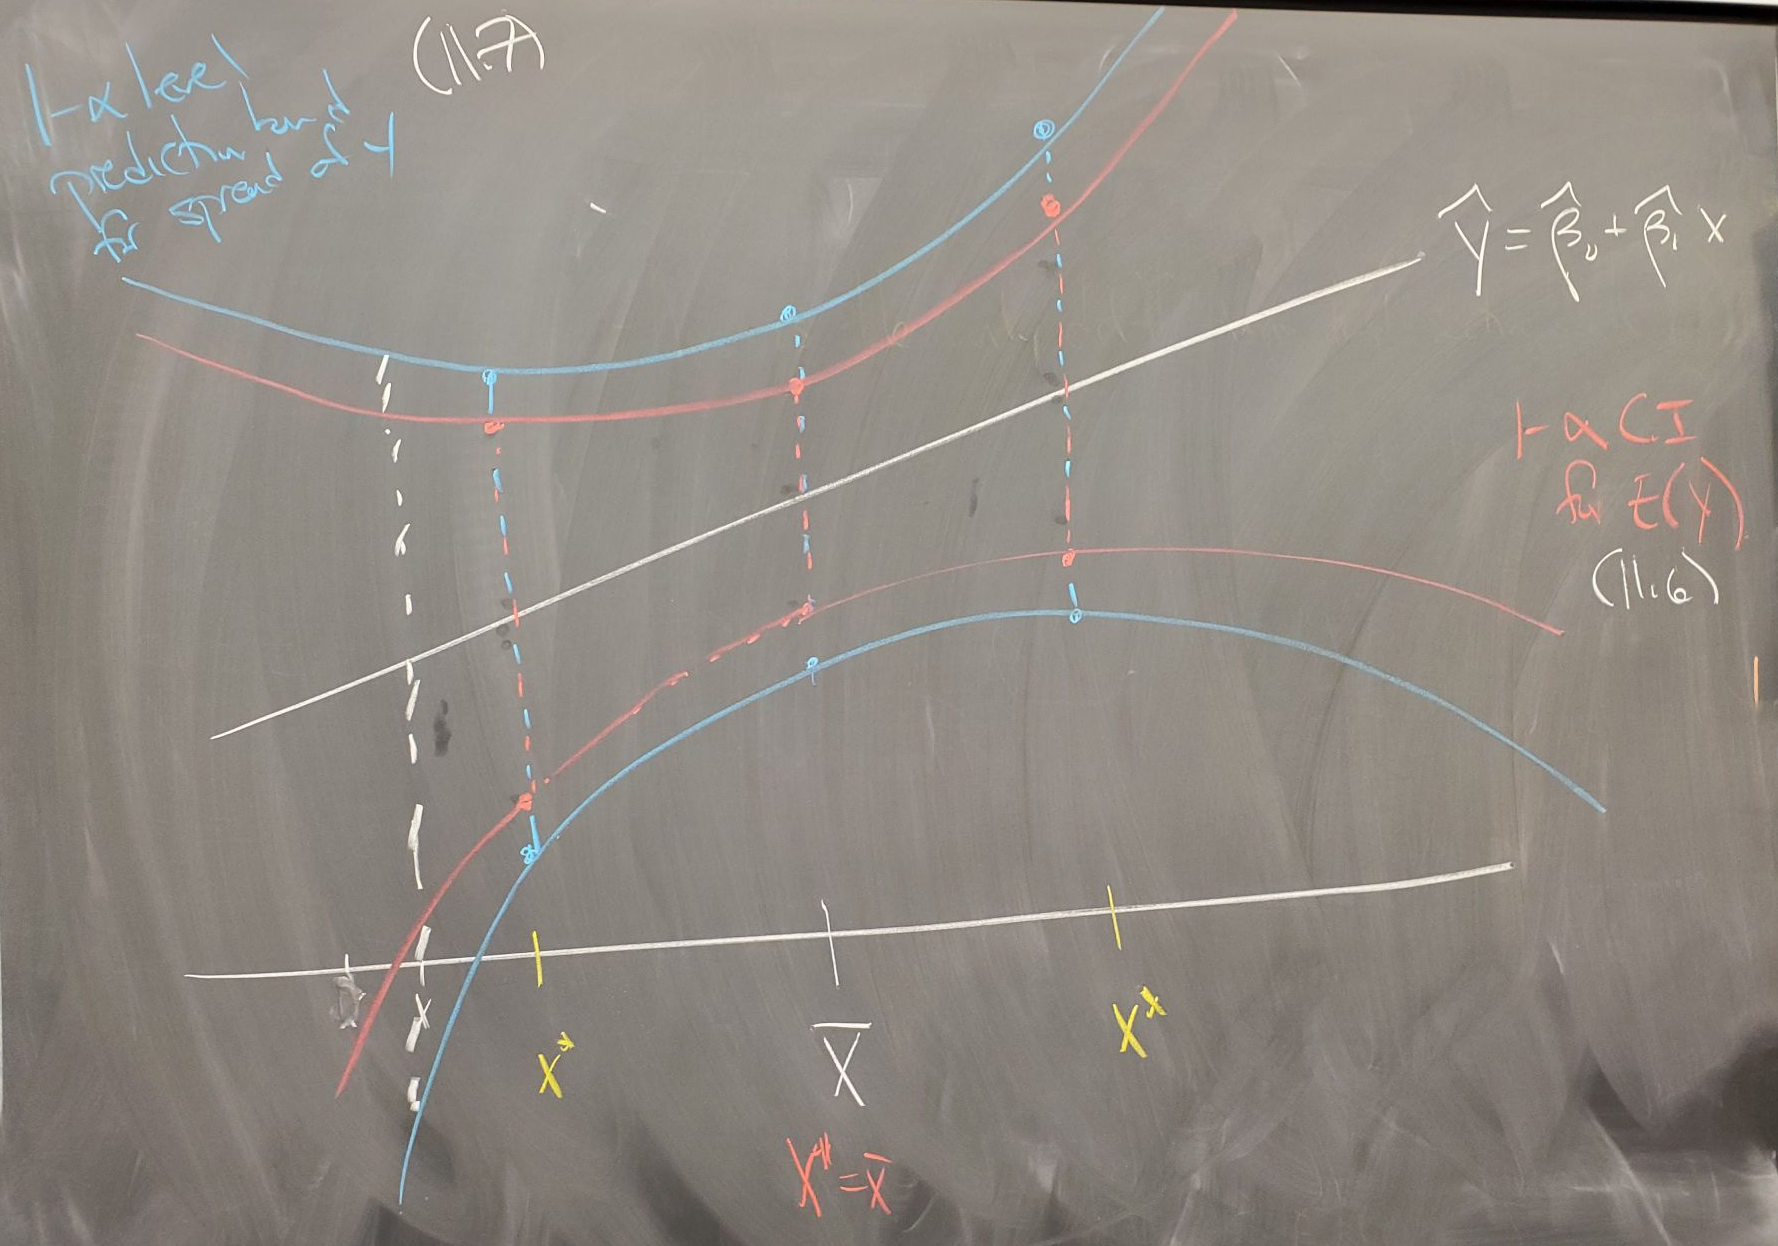
\includegraphics[width=6.5in]{11_7_hyperbola.png}
\end{center}

\noindent \textbf{Example: } Potency of antibiotic when stored at $20^{\circ}$F. Last day we showed that $\E{\widehat y(20)}$ had 90\% confidence interval
$$\setRed \underbrace{\setBlack 39.6 \pm 4.677}_{\text{red cross-section}}$$
What spread of potency would we expect to see with 90\% confidence if stored at $20^{\circ}$F. The same calculation as the last but with new standard error 
$$39.\overline6 \pm 1.812 \sqrt{1 + \over{12} + \frac{1600}{6000}}$$
$$\setBlue \underbrace{\setBlack 39.6 \pm 5.069}_{\text{blue cross-section}}$$



\setSection{9}
\section{Multiple Linear Regression}
\textbf{\color{eblue}Example: } Consider the data:
  \begin{center}
    \begin{tabular}{|l|c|c|c|c|c|} 
         \hline
         $x$ & -1 & 1 & 2 & 3\\
         \hline 
         $y$ & 0.5 & -1 & -0.5 & 2\\
         \hline
    \end{tabular}
\end{center}
The the plot does not look linear:
\begin{center}
    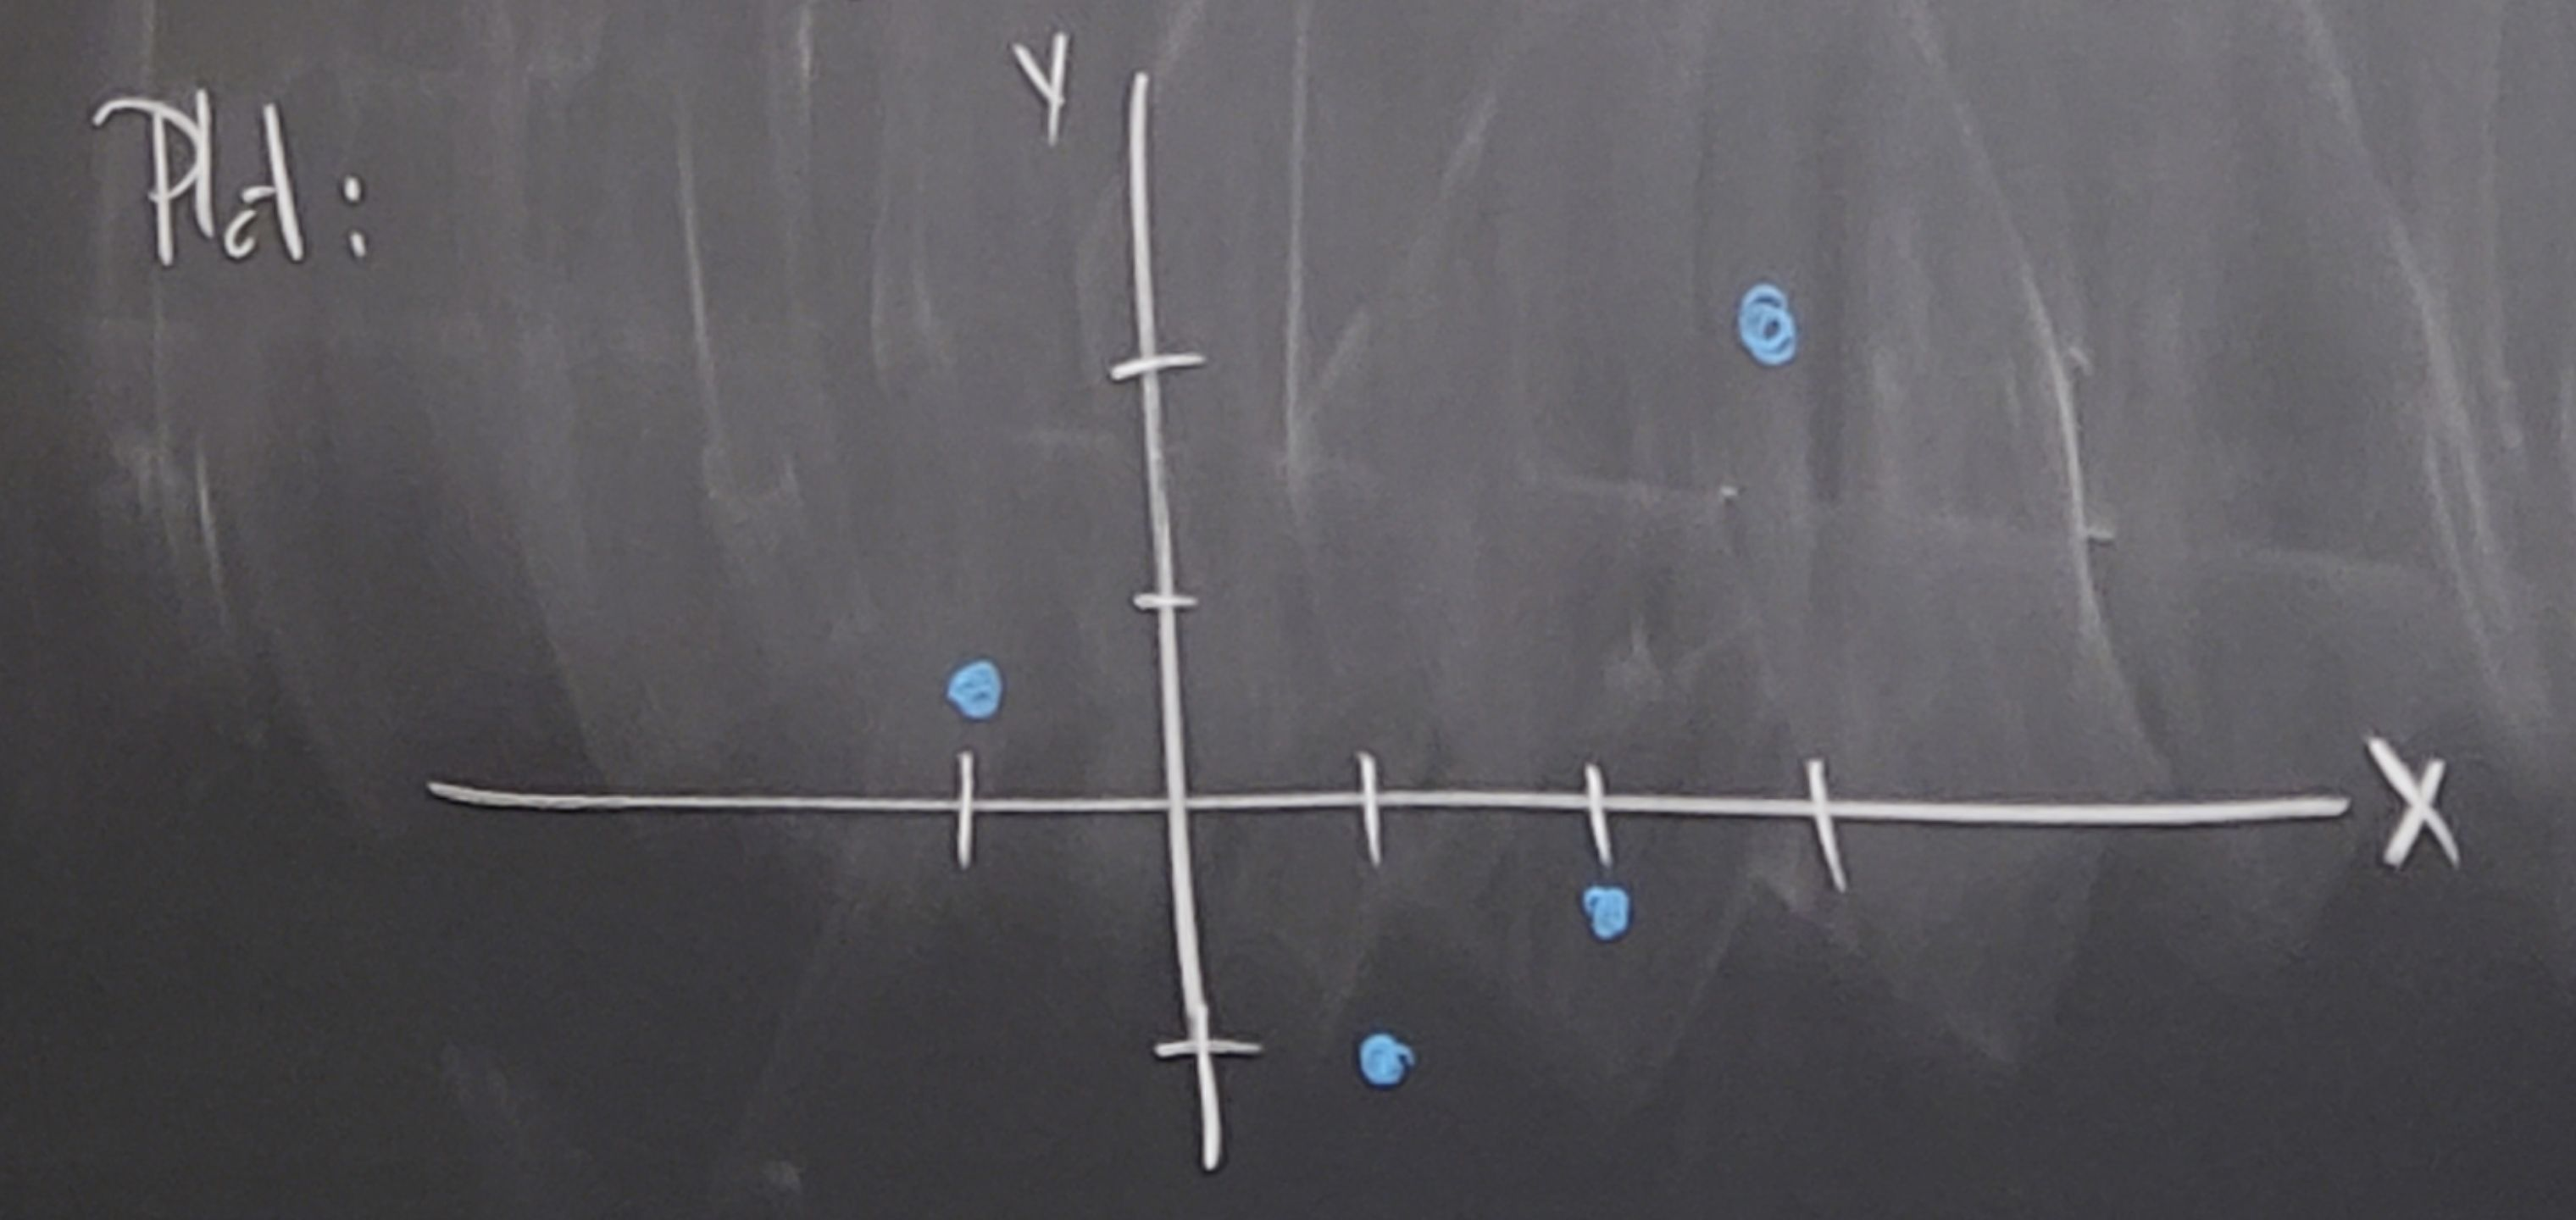
\includegraphics[height=2in]{11_10 plot.jpg}
\end{center}

\nl Seems unlikely that a line will fit well. What about a parabola? Want $y = \beta_0 + \beta_1x + \beta_2x^2$. Of course, in the probabilistic setup:
$$y = \underbrace{\beta_0 + \beta_1x + \beta_2x^2}_{\text{deterministic}} + \setRed \underbrace{ \varepsilon}_{\text{error}}$$
Using the data:
\begin{align*}
    \over{2} &= \beta_0 + \beta_1(-1) + \beta_2(-1)^2\\
    -1 &= \beta_0 + \beta_1(1) + \beta_2(1)^2 \\
    -\over{2} &= \beta_0 + \beta_1(2) + \beta_2(2)^2\\
    2 &= \beta_0 + \beta_1(3) + \beta_2(3)^2
\end{align*}
But this is the same idea as before, just in higher dimensions (3 coefficents).
$$\vec y = \beta_0 \vec 1 + \beta_1 \vec x + \beta_2 \vec{x^2}$$
$$= \beta_0 \begin{pmatrix}
    1\\1\\1\\1
\end{pmatrix} + \beta_1 \begin{pmatrix}
    -1\\1\\2\\3
\end{pmatrix} + \beta_2 \begin{pmatrix}
    1\\1\\4\\9
\end{pmatrix}$$
Or, as a matrix equation,
$$\begin{bmatrix}
    1 & -1 & 1\\ 1 & 1 & 1 \\ 1 & 2 & 4 \\ 1 & 3 & 9
\end{bmatrix} \begin{bmatrix}
    \beta_0 \\ \beta_1 \\ \beta_2
\end{bmatrix} = \begin{bmatrix}
    1/2 \\ -1 \\ -1/2 \\ 2
\end{bmatrix}.$$
Remark: This is why this process is called \textbf{linear} regression.

\nl The system for the coefficients will be a linear system. It has \red{nothing} to do with the underlying model\dots WHich here is quadratic $y = \beta_0 + \beta_1 x + \beta_2 x^2$.

\nl Just as before, we have an overdetermined system, which implies there is no solution. Hence, the best we can do is find the projection.

\nl We need a way to solve this projection problem in general. 

\nnl \textbf{Topic: The Normal Equations: }\\
In complete generality, $$y = \beta_0 + \beta_1 f_1(x) + \beta_2 f_2(x) + \cdots + \beta_n f_n(x) + \varepsilon.$$
Let there be $m$ data points $(x_i, y_i)$.

\nl This yields a matrix equation:
$$\begin{bmatrix}
    1 & f_1(x_1) & f_2(x_1) & \cdots & f_n(x_1)\\
    1 &  f_1(x_2) & f_2(x_2) & \cdots & f_n(x_2)\\
    \vdots & \vdots & \vdots & \ddots & \vdots \\
    1 &  f_1(x_n) & f_2(x_n) & \cdots & f_n(x_n)\\
\end{bmatrix} \begin{bmatrix}
    \beta_0 \\ \beta_1 \\ \vdots \\ \beta_n
\end{bmatrix} = \begin{bmatrix}
    y_1\\ y_2 \\ \vdots \\ y_n
\end{bmatrix}$$
Write $\mathbf X \vec{\beta} = \vec y$. Then $\mathbf X$ is $m$x$n$.

\nl Note, this setup really only makes sense when the system is overdetermined (more equations than unknowns). That is, more rows then columns in $\mathbf X$. i.e. $m > n$. We seek the coefficient vectors $\widehat{\beta} = [\thru{\widehat{\beta}}]$ such that $\norm{y - \mathbf X \widehat{\beta}}$ is minimized (LSR).

\nl In the gernal case, there are 2 new issues to content with:
\begin{enumerate}[label=\textcircled{\raisebox{-1pt}{\arabic*}}]
    \item no reason the column vectors of $\mathbf X$ are actually a basis for $\operatorname{Col} \mathbf X (might just be a spanning set)$.
    \item Certainly no reason columns are an orthogonal set. 
\end{enumerate}
The implication of $\textcircled{\raisebox{-1pt}{1}}$ is that a least squares solution $\widehat{\beta}$ need not be unique. As for $\textcircled{\raisebox{-1pt}{2}}$, ends we don't need this. By definition $\vec y - \mathbf X \widehat{\beta}$ is orthogonal to $\operatorname{Col}\mathbf X$.

\nl In other words, $\vec y - \mathbf X \widehat{\beta}$ must lie in the null space of $\mathbf X ^T$. (Recall $(\operatorname{Col} )^{\perp} = \operatorname{null}A^T$).

\nl Thus, $\mathbf X^T (y - \mathbf X \widehat{\beta}) = \vec 0$. 
$$\implies \underbrace{\mathbf X^T y}_{m \text{ vector}} - \underbrace{\mathbf X^T \mathbf X \widehat{\beta}}_{m \text{ vector}} = \underbrace{0}_{m}$$
$$\implies \mathbf X^T \mathbf X \widehat{\beta} = \mathbf X^T y$$
Definition: The normal equations:
$$\mathbf X^T \mathbf X \widehat{\beta} = \mathbf X^T y$$

\nl Facts:
\begin{enumerate}[label=\textcircled{\raisebox{-1pt}{\arabic*}}]
    \item $\mathbf X^T \mathbf X$ is an $n$x$n$ matrix.
    \item The normal equation is always a consistent system. That is, there is a solution to the least squares problem.
    \item If the columns of $\mathbf X$ are linearly independent, then $\mathbf X^T \mathbf X$ is an invertible square matrix and the unique solution to the least squares problem is
    $$\widehat{\beta} = \pars{\mathbf X^T \mathbf X}^{-1}\mathbf X^T y$$ 
\end{enumerate}

\example Our best fit parabola. 

$$\mathbf X = \begin{bmatrix}
    1 & -1 & 1\\ 1 & 1 & 1 \\ 1 & 2 & 4 \\ 1 & 3 & 9
\end{bmatrix}, \qquad \mathbf X^T = \begin{bmatrix}
    1 & 1 & 1 & 1\\ -1 & 1 & 2 & 3 \\ 1 & 1 & 4 & 9
\end{bmatrix}$$
$$\widehat{\beta} = [\widehat{\beta}_0, \widehat{\beta}_1, \widehat{\beta}_2], \quad y = \brac{ \over{2}, -1, -\over2, 2 }$$
$$\mathbf X^T \mathbf X = \begin{bmatrix}
    4 & 5 & 15\\ 5 & 15 & 35 \\ 15 & 35 & 99
\end{bmatrix}$$
Note that $\operatorname{det} (\mathbf X^T \mathbf X ) = 440 \neq 0$ so it is invertible. 
\begin{align*}
    \widehat{\beta} &= (\mathbf X^T \mathbf X )^{-1} \mathbf X^T y\\
    &= \begin{bmatrix}
        -41/44\\ -379/440 \\ 53/88
    \end{bmatrix}
\end{align*}
So, the best-fit parabola is 
\begin{align*}
    y &= -\frac{41}{44} - \frac{379}{440}x + \frac{53}{88}x^2\\
    &\approx -0.932 - 0.861x +0.602x^2
\end{align*}


\disc{Revisit the best-fit line}

\nl Given $n$ $(x_i,\, y_i)$'s, $y = \beta_0 + \beta_1 x + \varepsilon$. 
$$\implies \begin{bmatrix}
    \vec 1 & \bar x
\end{bmatrix} \widehat{\beta} = \vec y \wideand \widehat{\beta} = \begin{bmatrix}
    \widehat{\beta}_0\\ \widehat{\beta}_1
\end{bmatrix}$$
Here $\mathbf X = \begin{bmatrix}
    \vec 1 & \bar x
\end{bmatrix}$ is a $n\,\text{x}\,2$ matrix and $\mathbf X^T = \begin{bmatrix}
    1^T\\ x^T
\end{bmatrix}$ is $2\,\text{x}\,n$.

\nl Then
\begin{align*}
    \mathbf X^T \mathbf X &= \begin{bmatrix}
        1^T\\ x^T
    \end{bmatrix} \begin{bmatrix}
        \vec 1 & \bar x
    \end{bmatrix}\\
    &= \begin{bmatrix}
        1 \cdot 1 & 1 \cdot x\\ x \cdot 1 & x \cdot x \end{bmatrix}\\
        &= \begin{bmatrix}
            n & \sum x_i\\ \sum x_i & \sum {x_i}^2
        \end{bmatrix}
\end{align*}
Normal equation $X^TX \widehat{\beta} = X^T y$. Can we solve uniquely? 

\begin{align*}
    \det (X^TX) &= n \sum {x_i}^2 - \pars{\sum x_i}^2\\
    &= n \sum {x_i}^2 - n^2 \bar x^2\\
    &= n \pars{\sum {x_i}^2 - n \bar x}\\
    &= n S_{xx}\\
    &>0
\end{align*}
Therefore $X^TX$ is invertible! ($\det A \ne 0 \iff A^{-1}$ exists)

\nl So $\widehat{\beta} = (X^TX)^{-1}X^Ty$

\recall* $\displaystyle \begin{bmatrix}
    a & b \\ c & d
\end{bmatrix}^{-1} = \over*{\det A} \bigbrac{(\operatorname{tr}A)I - A} = \over{ad-bc} \begin{bmatrix}
    d & -b\\ -c & a
\end{bmatrix}$.

\nl So $$\displaystyle (X^TX)^{-1} = \over{nS_{xx}} \begin{bmatrix}
    \sum {x_i}^2 & - \sum x_i \\  - \sum x_i & n
\end{bmatrix} $$
and
$$X^T y = \begin{bmatrix}
    1^T \\ x^T
\end{bmatrix} y = \begin{bmatrix}
    1 \cdot y \\ x \cdot y
\end{bmatrix} = \begin{bmatrix}
    \sum y_i\\ \sum x_i y_i
\end{bmatrix}$$
Then
\begin{align*}
    \widehat{\beta} &= \over{nS_{xx}} \begin{bmatrix}
        \sum {x_i}^2 & - \sum x_i\\ -\sum x_i & n
    \end{bmatrix} \begin{bmatrix}
        \sum y_i \\ \sum x_i y_i
    \end{bmatrix}
    \\
    &= \over{n S_{xx}} \begin{bmatrix}
        (\sum {x_i}^2)(\sum y_i) - (\sum x_i)(\sum x_i y_i)\\
        -(\sum x_i)(\sum y_i) + n \sum x_i y_i
    \end{bmatrix}
\end{align*}
Same $\widehat{\beta}_0, \widehat{\beta}_1$ as earlier. But wait there's more\dots, Look at $(X^TX)^{-1}$:
\begin{align*}
    (X^TX)^{-1} &= \over{nS_{xx}} \begin{bmatrix}
        \sum {x_i}^2 & -n \bar x\\ -n \bar x & n
    \end{bmatrix}\\
    &= \begin{bmatrix}
        \dfrac{\sum {x_i}^2}{n S_{xx}} & -\dfrac{\bar x}{S_{xx}}\\ -\dfrac{\bar x}{S_{xx}} & \dfrac{1}{S_{xx}}
    \end{bmatrix}
\end{align*}
And
\begin{align*}
    \sigma^2 (X^TX)^{-1} &= \begin{bmatrix}
        \Var{\betah_0} & \Cov (\betah_0, \betah_1)
        \\ \Cov (\betah_0, \betah_1)  & \Var{\betah_1}
    \end{bmatrix}
\end{align*}
\textbf{FACT:} This always happens. $\sigma^2 (X^TX)^{-1}$ is the table of covariances:
$$\sigma^2 - a_{i\,j} = \Cov (\betah_i, \betah_j) \quad \text{where} \quad [a_{i\,j}] = (X^TX)^{-1}$$
Lastly,
$$S^2 = \frac{\operatorname{SSE}}{n-2} = \frac{\displaystyle \sum (y_i - \widehat{y}_i)^2}{n-2}$$
And \say{by some matrix algebra} (Wackerly),
$$\operatorname{SSE} = y^Ty - \betah^T \mathbf X^T y.$$

\example* (Antibiotic again)
\begin{center}
    \begin{tabular}{|l||c|c|c|c|c|c|c|c|c|c|c|c|} 
         \hline
         $x$ & 30 & 30 & 30 & 50 & 50 & 50 & 70 & 70 & 70 & 90 & 90 &90 \\
         \hline 
         $y$ & 38 & 43 & 29 & 32 & 26 & 33 & 19 & 24 & 23 & 14 & 19 & 21\\
         \hline
    \end{tabular}
\end{center}
$n = 12$ and $X^TX \displaystyle = \bmat{n}{\sum x_i}{\sum x_i}{\sum {x_i}^2} = \bmat{12}{720}{720}{\num{49200}}$. Then $\det (X^TX) = \num{72000}$. Then
$$(X^TX)^{-1} = \over{\num{72000}} \begin{bmatrix}
    \num{49200} & -700 \\ -700 & 12
\end{bmatrix}.$$
\setRed \textbf{Note:} \setBlack $\Var*{\betah_0} = \dfrac{41}{60}\sigma^2$, and $\Var*{\betah_1} = \dfrac{\sigma^2}{6000}$. 

\nl Then $X^Ty \displaystyle = \vvec*{\sum y_i}{\sum x_iy_i} = \vvec*{324}{\num{17540}}$ and $\betah = (X^TX)^{-1}X^Ty = \vvec*{46}{-19/60}$ (same as before). Hence 
$$\widehat{y} = 46 - \frac{19}{60}x$$
$$\operatorname{SSE} = y^Ty - \betah^T X^Ty = \frac{2961}{15}$$
$$\sigma^2 \approx \frac{\operatorname{SSE}}{n-2} = \frac{2971/15}{10} \approx 19.8067.$$
\section{A big ol theorem}

\nl Theorem: Let $Y_i = \beta_0 + \beta_1 f_1(x_i) + \cdots + \beta_k f_k (x_i) + \varepsilon_i$ where $\varepsilon_i \sim \normalDist{0, \sigma^2}$ (with $\Eb{\varepsilon} = 0$).

\nl Then the least-squares estimates are given by $\widehat{\beta} = (X^TX)^{-1}X^Ty$ provided $(X^TX)^{-1}$ exists. Then 

\begin{enumerate}[label=\textcircled{\raisebox{-1pt}{\arabic*}}]
    \item $\E*{\betah_i} = \betah_i \qquad \text{(unbiased)}$
    \item $\Var*{\betah_1} = c_{i\,i} \sigma^2$ \hspace{.2in} where $(X^TX)^{-1} = [c_{i\,j}]$
    \item $\Cov(\betah_i, \betah_j) = c_{i\,j} \sigma^2$
    \item $S^2 = \dfrac{\operatorname{SSE}}{n-(k+1)}$ \hspace{.1in} with $k+1 \; \betah_i$'s and $\operatorname{SSE} = y^Ty - \betah^T X^Ty$ and $\E{S^2} = \sigma^2$ (unbiased)
    \item $\betah_i$ is normally distributed.
    \item $\dfrac{(n-(k+1))S^2}{\sigma^2} \sim \chi^2(n-(k+1))$
    \item $S^2$ and $\betah_1$ are independent for all $i$.
\end{enumerate}
\section{Hypothesis Testing C.I.}
Motivation: Testing a specific $\betah_i$.

\nl We have $\betah = (X^TX)^{-1}Ty = [\betah_0, \dots, \betah_k]$. To pick off a specific $\betah_i$, we use the dot product.

\nl Let $e_i$ (standard basis vector), then $\displaystyle \betah_i = \underbrace{e_i \cdot \betah}_{\text{dot product}} = \underbrace{{e_i}^T \betah}_{\substack{\text{matrix} \\ \text{multiplication}}}$

\nl Note: $\E*{e_i \cdot \betah} = \E*{1 \cdot \betah_i} = \E*{\betah_i} = \beta_i$.
\\ Same with $\Var*{e_i \cdot \betah} = \Var*{\betah_i}$.

\nl So a test of the form
\begin{align*}
    H_0 &: \betah_i = (\beta_i)_0\\
    H_a &: \betah_i \neq (\beta_i)_0
\end{align*}
yields same old statistics.
$$Z = \frac{\betah_i - (\beta_i)_0}{\sqrt{\Var*{\beta_i}}} = \frac{\betah_i - (\beta_i)_0}{\sqrt{c_{i\,i}\sigma^2}} \qquad \text{with} \qquad [c_{i\,i}] = (X^TX)^{-1}$$
$$T = \frac{\betah_i - (\beta_i)_0}{S \sqrt{c_{i\,i}}} \qquad \text{with} \qquad n-(k+1) \text{ df.}$$

\example*
We fit
\begin{center}
    \begin{tabular}{|l|c|c|c|c|c|}
         \hline
         $x$ & -1 & 1 & 2 & 3\\
         \hline
         $y$ & 0.5 & -1 & -0.5 & 2\\
         \hline
    \end{tabular}
\end{center}
with $y = \beta_0 + \beta_1 x + \beta_2 x^2$ because it \say{looked} non-linear.
\begin{center}
    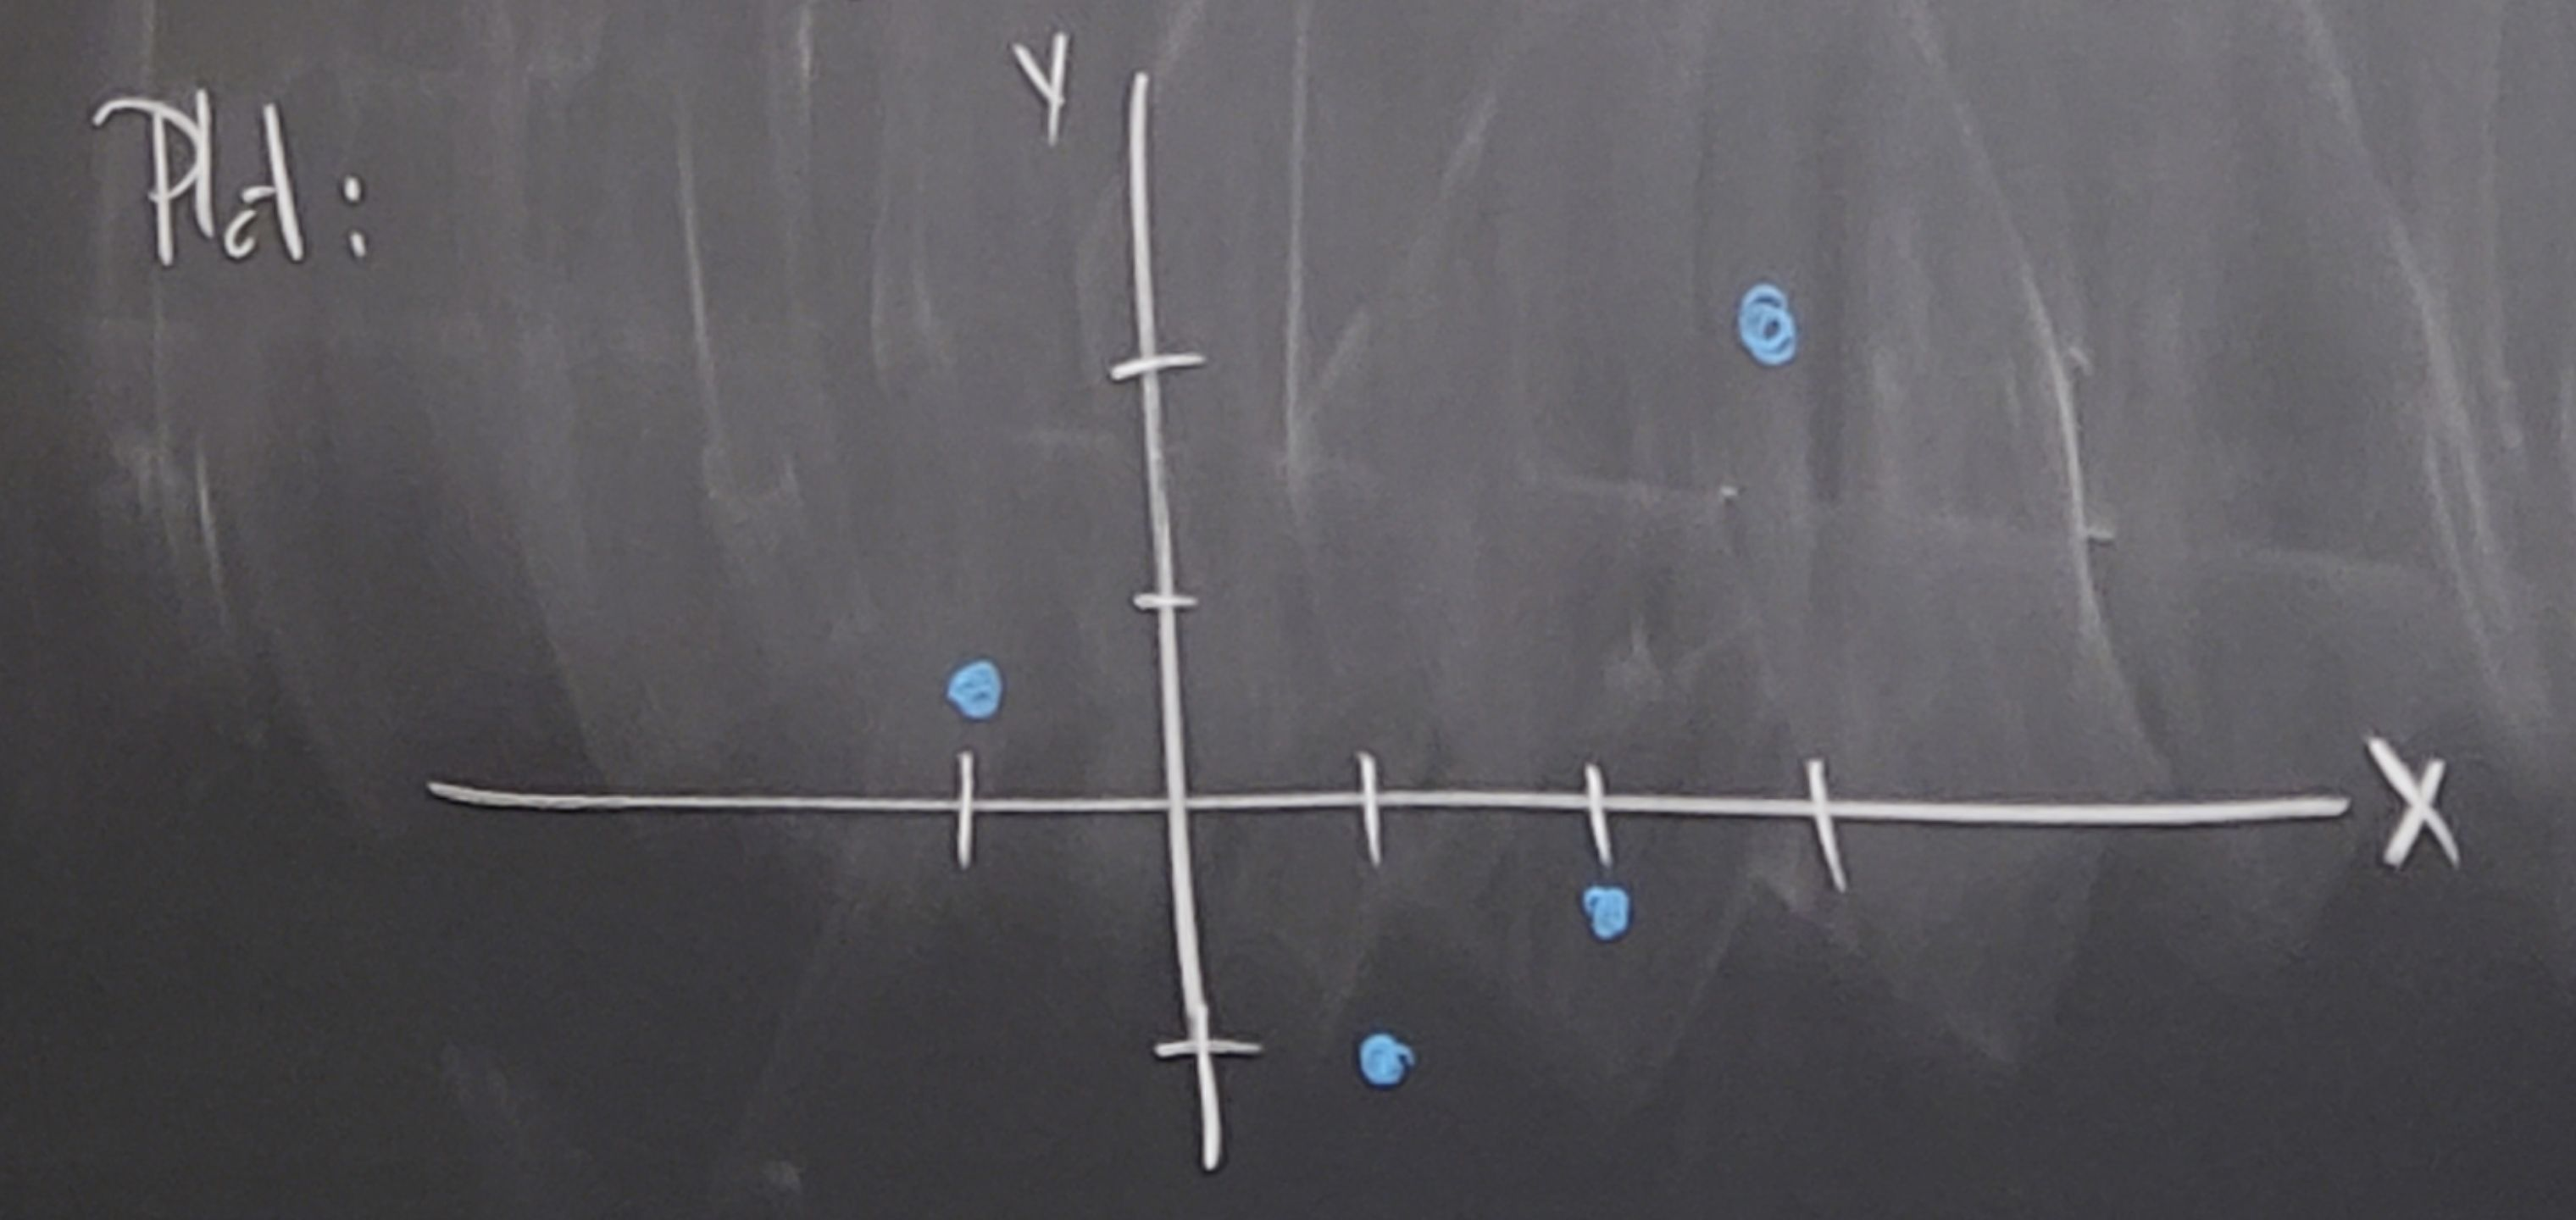
\includegraphics[height=2in]{11_10 plot.jpg}
\end{center}
Is there evidence that the data is in fact non-linear? That is, are we reasonably certain $\beta_{\alpha} \neq 0$.
\begin{align*}
    H_0 &: \beta_{\alpha} = 0\\
    H_a &: \beta_{\alpha} \neq 0
\end{align*}
We had
\begin{align*}
    \widehat{\beta} &= (\mathbf X^T \mathbf X )^{-1} \mathbf X^T y\\
    &= \begin{bmatrix}
        -41/44\\ -379/440 \\ 53/88
    \end{bmatrix}\\
    &= \vvec*{\betah_0}{\betah_1}{\betah_2}
\end{align*}
$e_3 = (0,0,1)$ and ${e_3}^T\betah = \dfrac{53}{80}$. We had
$$\mathbf X^T \mathbf X = \begin{bmatrix}
    4 & 5 & 15\\ 5 & 15 & 35 \\ 15 & 35 & 99
\end{bmatrix}$$
and $\det (\mathbf X^T \mathbf X) = 440$. Then
$$(\mathbf X^T \mathbf X)^{-1} = \over{440} \begin{bmatrix}
    260 & 30 & -50 \\
    30 & 171 & -65\\
    -50 & -65 & 35
\end{bmatrix}$$
With $\Var*{\betah_2} = c_{2\,2} \sigma^2 = \dfrac{35}{440}\sigma^2$. % was this beta2?

\nl For $\sigma^2$, we need $S^2 = \dfrac{\operatorname{SSE}}{n-2}$.
$$\operatorname{SSE} = y^Ty - \betah^T X^Ty = \frac{4791}{440}.$$
$$S^2 = \frac{\frac{4791}{440}}{n-2} = \frac{4791}{850} \approx 5.44432.$$
$$\Var*{\betah_2} \approx c_{2\,2} S^2 \cdots \sqrt{\Var*{\betah_2}} = 0.690201.$$
So
\begin{align*}
    T &= \frac{e_3 \cdot \betah - (\betah_2)_0}{\sqrt{\Var*{\betah_2}}}\\
    &= \frac{\frac{53}{88}-0}{0.690201}\\
    &= 0.872604
\end{align*}
$$\P{\abs{T} \geq 0.872604 \mid \df = 2} = 0.4748909.$$
\red{This sucks! It supports the null Hypothesis.}

\example* (Potency again)
\begin{center}
    \begin{tabular}{|l||c|c|c|c|c|c|c|c|c|c|c|c|}
         \hline
         $x$ & 30 & 30 & 30 & 50 & 50 & 50 & 70 & 70 & 70 & 90 & 90 &90 \\
         \hline
         $y$ & 38 & 43 & 29 & 32 & 26 & 33 & 19 & 24 & 23 & 14 & 19 & 21\\
         \hline
    \end{tabular}
\end{center}
I tried quadratic $y = \beta_0 + \beta_1x + \beta_2x^2$.
$$X = \begin{bmatrix}
    1 & x & x^2
\end{bmatrix}$$
$$(X^TX)^{-1} = \over{1.92 \times 10^6} \begin{bmatrix}
    1.092 \times 10^6 & -391200 & 3100\\
    -391200 & 14720 & -120\\
    3100 & -120 & 1
\end{bmatrix}$$
Note: $\Var*{\betah_2} = \over*{1.92 \times 10^6}\sigma^2 \approx \dfrac{S^2}{1920000}$.
$$\operatorname{SSE} = y^Ty + \betah^TX^Ty = 189.$$
$$S^2 = \frac{\operatorname{SSE}}{n-2} = \frac{\operatorname{SSE}}{10} = 18.9$$
$$\Var*{\betah_2} = 9.84775 \times 10^{-6}.$$
$$\sqrt{\Var*{\betah_2}} = 0.00313748$$
Testing
\begin{align*}
    H_0 &: \beta_2 = 0\\
    H_a &: \beta_2 \neq 0
\end{align*}
I computed $\betah_2 = \over*{1200}$.
$$t = \frac{\betah_2 - (\beta_2)_0}{\sqrt{\Var*{\betah_2}}} = 0.2656$$
With $\df = 10$, $\P{\abs{T} > 0.2656} = 0.79$, which is HUGE again. Hence it supports the null hypothesis.

\nl Of course, this is a math class and we love to generalive. We don't have to use a standard basis vector $e_i$. Let $\vec{a}$ be a constant vector $a = (a_0, \dots, a_k)$. Then
$$a^T\betah = a_0 \betah_0 + \dots + a_k \betah_k.$$
Note:
\begin{align*}
    \E*{a^T \betah} &= \sum{i=1}^k a_i \E*{\betah_i} \tag{by linearity}\\
    &= \sum{i=1}^k a_i \beta_i \tag{by unbiases estimators}\\
    &= a^T \beta
\end{align*}
for $\beta = (\beta_0, \dots, \beta_k)$. Also,
\begin{align*}
    \Var*{a^T \betah} &= \Var*{a_0 \betah_0 + \cdots + a_k \betah_k}\\
    &= \sum{i=1}^k \sum{j=1}^k \Cov (a_i \betah_i, a_j \betah_j)\\
    &= \sum{i=1}^k \sum{j=1}^k a_i a_j \underbrace{\Cov (\betah_i, \betah_j)}_{\substack{\text{These are } c_{i\,j} \sigma^2 \text{'s} \\ \text{from } (X^TX)^{-1}}}
\end{align*}
This entire double sum can be written as the matrix product
$$\Var*{a^T \betah} = a^T (X^TX)^{-1}a \cdot \sigma^2$$
% = 1xk, kxk, kx1
$$\implies Z = \frac{a^T \betah - \E{a^T \betah}}{\Var{a^T\betah}} = \frac{a^T \betah - a^T \beta}{\sigma \sqrt{a^T (X^TX)^{-1} a} }$$

\nl Given $H_0 : a^T \beta = (a^T \beta)_0$ versus some alternative, use
$$T = \frac{a^T \betah - (a^T \beta)_0}{S \sqrt{a^T (X^TX)^{-1}a}}$$
with $n-(k+1)$ degrees of freedom. 